%\documentclass[handout]{ximera}
\documentclass[nooutcomes]{ximera}

\usepackage{gensymb}
\usepackage{tabularx}
\usepackage{mdframed}
\usepackage{pdfpages}
%\usepackage{chngcntr}

\let\problem\relax
\let\endproblem\relax

\newcommand{\property}[2]{#1#2}




\newtheoremstyle{SlantTheorem}{\topsep}{\fill}%%% space between body and thm
 {\slshape}                      %%% Thm body font
 {}                              %%% Indent amount (empty = no indent)
 {\bfseries\sffamily}            %%% Thm head font
 {}                              %%% Punctuation after thm head
 {3ex}                           %%% Space after thm head
 {\thmname{#1}\thmnumber{ #2}\thmnote{ \bfseries(#3)}} %%% Thm head spec
\theoremstyle{SlantTheorem}
\newtheorem{problem}{Problem}[]

%\counterwithin*{problem}{section}



%%%%%%%%%%%%%%%%%%%%%%%%%%%%Jenny's code%%%%%%%%%%%%%%%%%%%%

%%% Solution environment
%\newenvironment{solution}{
%\ifhandout\setbox0\vbox\bgroup\else
%\begin{trivlist}\item[\hskip \labelsep\small\itshape\bfseries Solution\hspace{2ex}]
%\par\noindent\upshape\small
%\fi}
%{\ifhandout\egroup\else
%\end{trivlist}
%\fi}
%
%
%%% instructorIntro environment
%\ifhandout
%\newenvironment{instructorIntro}[1][false]%
%{%
%\def\givenatend{\boolean{#1}}\ifthenelse{\boolean{#1}}{\begin{trivlist}\item}{\setbox0\vbox\bgroup}{}
%}
%{%
%\ifthenelse{\givenatend}{\end{trivlist}}{\egroup}{}
%}
%\else
%\newenvironment{instructorIntro}[1][false]%
%{%
%  \ifthenelse{\boolean{#1}}{\begin{trivlist}\item[\hskip \labelsep\bfseries Instructor Notes:\hspace{2ex}]}
%{\begin{trivlist}\item[\hskip \labelsep\bfseries Instructor Notes:\hspace{2ex}]}
%{}
%}
%% %% line at the bottom} 
%{\end{trivlist}\par\addvspace{.5ex}\nobreak\noindent\hung} 
%\fi
%
%


\let\instructorNotes\relax
\let\endinstructorNotes\relax
%%% instructorNotes environment
\ifhandout
\newenvironment{instructorNotes}[1][false]%
{%
\def\givenatend{\boolean{#1}}\ifthenelse{\boolean{#1}}{\begin{trivlist}\item}{\setbox0\vbox\bgroup}{}
}
{%
\ifthenelse{\givenatend}{\end{trivlist}}{\egroup}{}
}
\else
\newenvironment{instructorNotes}[1][false]%
{%
  \ifthenelse{\boolean{#1}}{\begin{trivlist}\item[\hskip \labelsep\bfseries {\Large Instructor Notes: \\} \hspace{\textwidth} ]}
{\begin{trivlist}\item[\hskip \labelsep\bfseries {\Large Instructor Notes: \\} \hspace{\textwidth} ]}
{}
}
{\end{trivlist}}
\fi


%% Suggested Timing
\newcommand{\timing}[1]{{\bf Suggested Timing: \hspace{2ex}} #1}




\hypersetup{
    colorlinks=true,       % false: boxed links; true: colored links
    linkcolor=blue,          % color of internal links (change box color with linkbordercolor)
    citecolor=green,        % color of links to bibliography
    filecolor=magenta,      % color of file links
    urlcolor=cyan           % color of external links
}

\title{Of Angles and Circles}
\author{Bart Snapp and Brad Findell}

\outcome{Learning outcome goes here.}

\begin{document}
\begin{abstract}
We study central and inscribed angles.
\end{abstract}
\maketitle

\begin{teachingnote}
A chord defines two central angles and two arcs: a ``standard'' and reflex angle pair, corresponding to a minor and a major arc.  So in this activity, central and inscribed angles intercept arcs rather than chords.
\end{teachingnote}

In this activity we are going to look at pictures and see if we can
explain how they ``prove'' theorems.

\begin{theorem} 
Any triangle inscribed in a circle and having the diameter as a side is a
right triangle.
\end{theorem}

\begin{problem}
Can you tell me in English what this theorem says? Provide some
examples of this theorem in action.
\end{problem}

\begin{problem} 
Here is a series of pictures, designed to be read from left to right.
\begin{image}
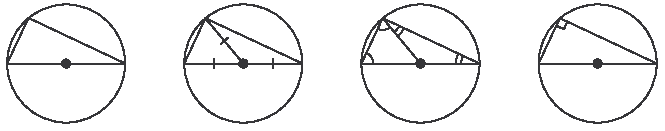
\includegraphics{pbpcircthm1.pdf}
\end{image}
Explain how these pictures ``prove'' the above theorem. In the process
of your explanation, you may need to label parts of the pictures and
do some algebra.
\end{problem}

\begin{definition}
A \emph{chord} in a circle defines two {arcs}, each of which corresponds to a {central angle}.  The \emph{measure} of the arc is defined to be the measure of the corresponding central angle.  
\end{definition}

\begin{problem}
Can you tell me in English what this definition says? Use pictures to demonstrate what the fancy words mean.  
\end{problem}

\begin{theorem} 
Given an arc of a circle, the central angle corresponding to this arc is
twice any inscribed angle intercepting this arc.
\end{theorem}

I'll play nice here and give you a picture of this theorem in action:
\begin{image}
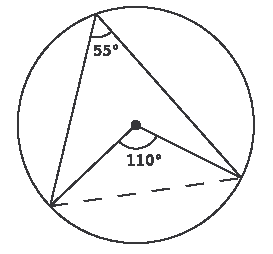
\includegraphics[scale=0.8]{pbpcircthm2eg.pdf}
\end{image}

\begin{problem}
Can you tell me in English what this theorem says?  Specifically, what is meant by
\textit{inscribed angle}?  And why does it say ``any inscribed angle''?
\end{problem}

\begin{problem} 
For one possible line of reasoning, consider this series of pictures, designed to be read from left to right.
\begin{image}
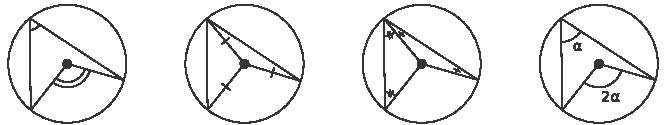
\includegraphics{pbpcircthm2.pdf}
\end{image}

Explain how these pictures ``prove'' the above theorem. In the process
of your explanation, you may need to label parts of the pictures and
do some algebra.
\end{problem}


\begin{problem}
Not all inscribed angles look like those in the previous picture.  Consider the following pictures:  
\begin{image}
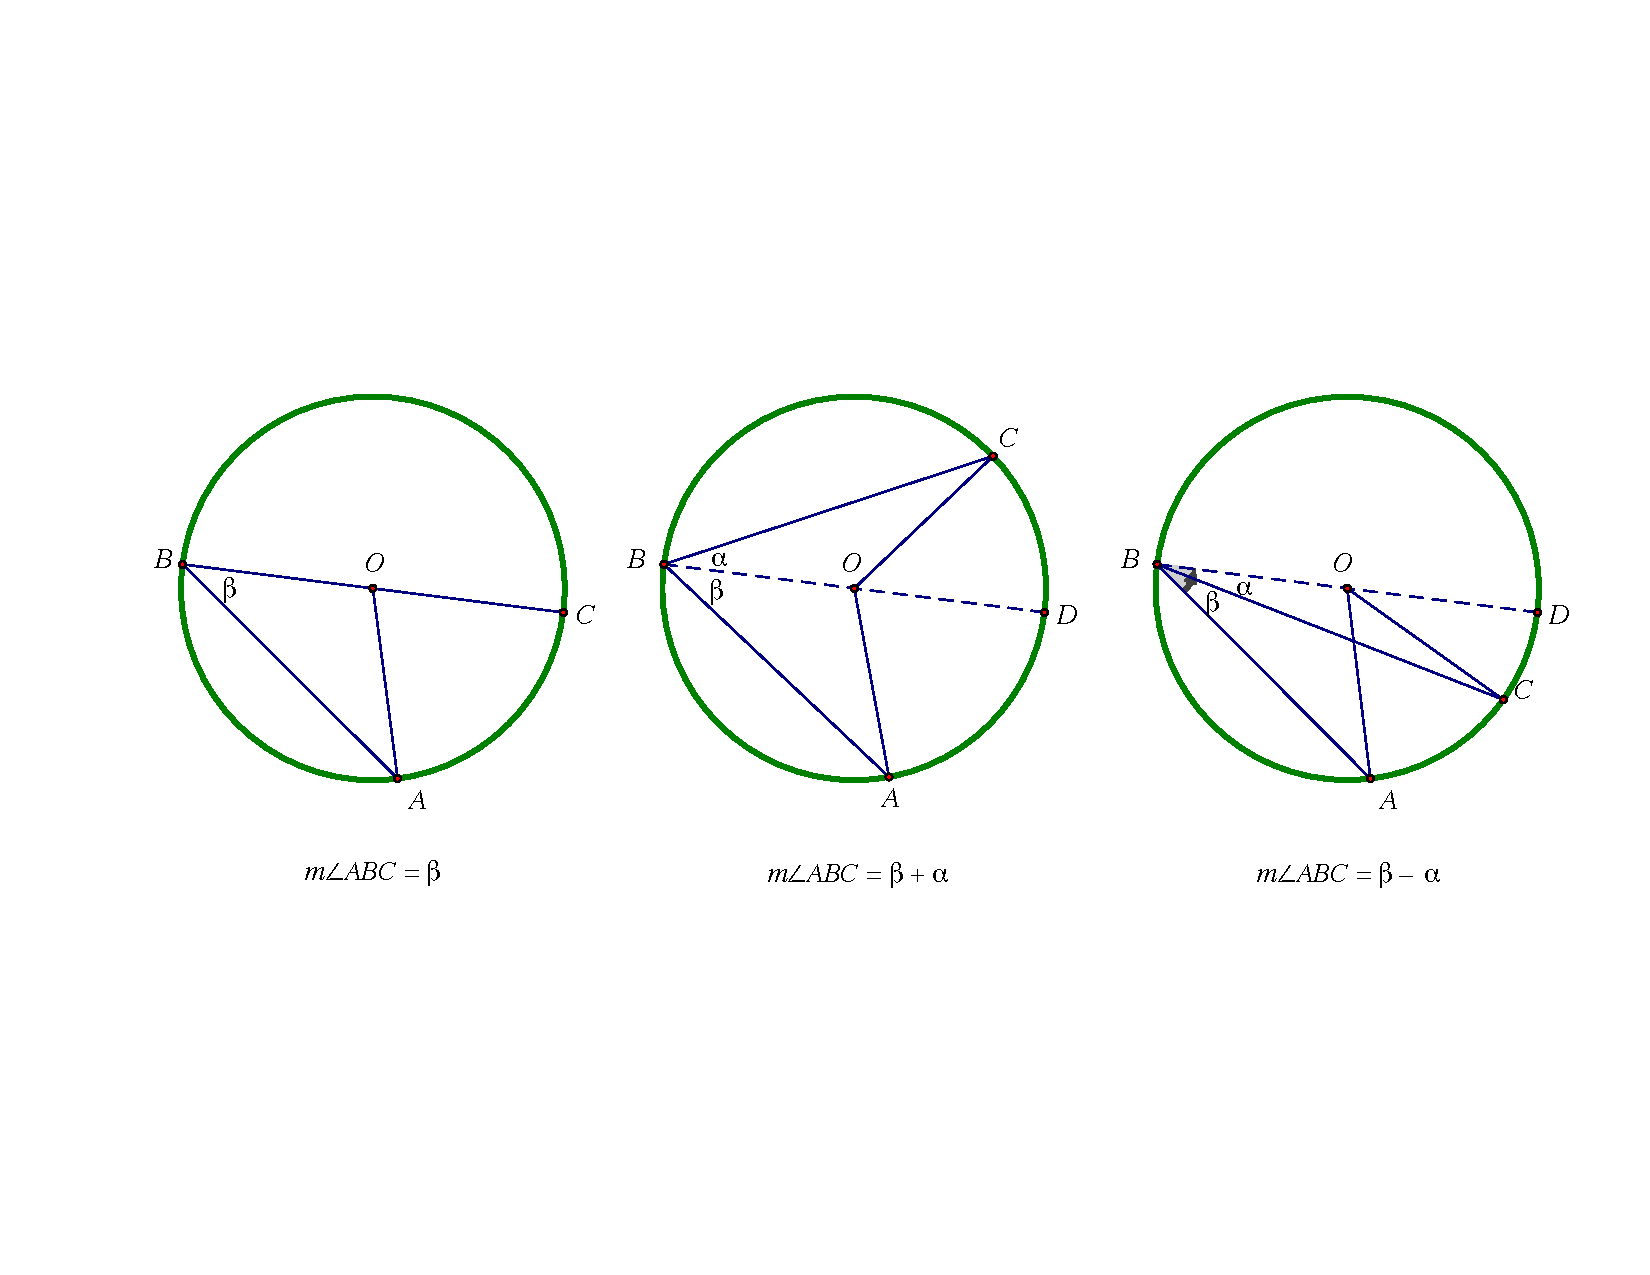
\includegraphics[width=5in]{inscribedAngle.pdf}
\end{image}
\
\begin{enumerate}
\item In each of the pictures, find and explain the relationship between $m\angle ABC$ and $m\angle AOC$.
\item Explain why any inscribed angle must fit one of these three cases.  
\end{enumerate}
% Can you show $m\angle AXB = \frac{1}{2}m\angle AOB$ for the sequence of cases below.  
\end{problem}

\begin{teachingnote}
The idea is rather simple, though it is not easy to see, especially in the third figure.  When the center is inside the inscribed angle, you can consider it to be the *sum* of two angles, each of which has one side through the center.  When the center is outside the inscribed angle, you can consider it to be the *difference* of two angles, each of which has one side through the center.  
\end{teachingnote}

\begin{corollary} 
Given an arc of a circle, all inscribed angles intercepting this arc are congruent.
\end{corollary}

\begin{problem} 
Firstly---what the heck is a corollary? Secondly---what is it saying?
Thirdly---why is it true?
\end{problem}
\end{document}
